\documentclass[10pt,a4paper]{article}
\usepackage[margin=20mm]{geometry}
\usepackage[T1]{fontenc}
\usepackage{lmodern}
\usepackage{microtype}
\usepackage{booktabs}
\usepackage{tabularx}
\usepackage{enumitem}
\usepackage{graphicx}
\usepackage{tikz}
\usepackage{xcolor}
\usepackage{hyperref}
\usetikzlibrary{arrows.meta,positioning}
\hypersetup{colorlinks=true,linkcolor=blue!45!black,urlcolor=blue!45!black}
\setlist{nosep,leftmargin=*}
\setlength{\parskip}{0.35em}
\setlength{\parindent}{0pt}
\title{Integrated PC UART Communication and Signal Tracing\\\large STM32 NUCLEO-H723ZG and NUCLEO-L476RG}
\author{Project Report}
\date{23 November 2026}

\begin{document}
\maketitle

\begin{abstract}
This report describes a two-board serial communication and observation system. An STM32 NUCLEO-H723ZG exchanges commands and acknowledgements with a PC over a UART link, operated by a small Python/Tkinter application. A separate STM32L476-based tracer board receives taps from the two UART signal directions and displays captured bytes on a serial console. The current source implements the H723 command protocol, variable baud-rate handshake, interrupt-driven tracer capture, and readable hexadecimal output. The report combines those implementations into one logical architecture and identifies the physical-layer checks and performance improvements needed for dependable integrated use.
\end{abstract}

\section{Purpose and project scope}
The project brings together two independently developed functions. The first is a PC-to-microcontroller link for sending repeatable test messages and receiving acknowledgements. The second is a passive UART monitor that distinguishes traffic travelling in each direction and makes binary data readable in a terminal. Together, they provide a practical bench setup for exercising a UART endpoint while observing the bytes on its communication link.

The H723 firmware initializes USART1 for 9600 baud, 8 data bits, no parity, one stop bit (8N1), and no hardware flow control. The PC connects through an FT232RL USB-to-UART adapter. The H723 TX and RX signals are also fed to the receive inputs of an STM32L476RG Nucleo tracer: USART1 RX and USART3 RX capture the two directions, while USART2 sends the trace to a PC serial monitor.

\section{System architecture}
Figure~\ref{fig:system} shows the actual signal flow. The FT232RL links the PC to H723 USART1. The two H723 UART signals are split to the L476 receive pins so the tracer can observe PC-to-H723 and H723-to-PC traffic while the original link remains active. The tracer sends its formatted output over its separate USART2 console connection to the PC serial monitor.

\begin{figure}[htbp]
\centering
\resizebox{0.94\linewidth}{!}{%
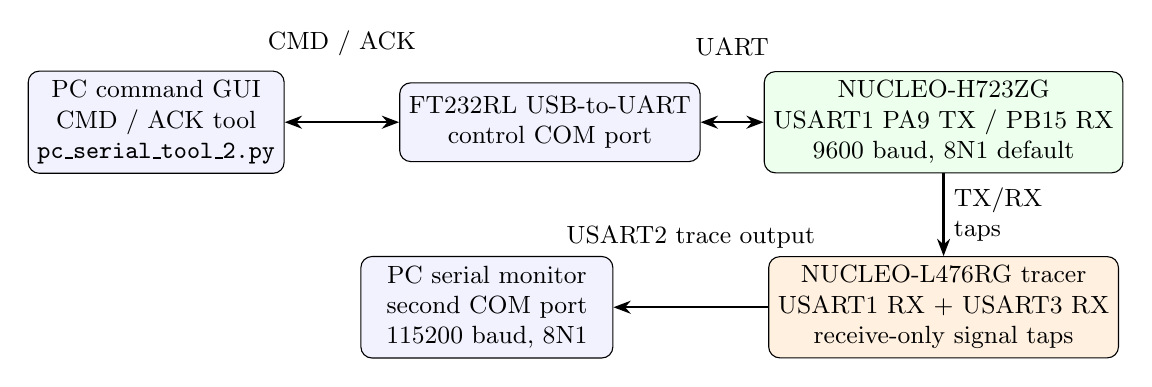
\begin{tikzpicture}[
  font=\small,
  unit/.style={draw,rounded corners,fill=blue!5,minimum width=3.2cm,minimum height=1.0cm,align=center},
  board/.style={draw,rounded corners,fill=green!7,minimum width=3.5cm,minimum height=1.15cm,align=center},
  tap/.style={draw,rounded corners,fill=orange!12,minimum width=3.6cm,minimum height=0.9cm,align=center},
  wire/.style={-{Stealth[length=2.2mm]},thick},
  bidir/.style={{Stealth[length=2.2mm]}-{Stealth[length=2.2mm]},thick}
]
\node[unit] (gui) at (0,2.35) {PC command GUI\\CMD / ACK tool\\\texttt{pc\_serial\_tool\_2.py}};
\node[unit] (adapter) at (5,2.35) {FT232RL USB-to-UART\\control COM port};
\node[board] (h723) at (10,2.35) {NUCLEO-H723ZG\\USART1 PA9 TX / PB15 RX\\9600 baud, 8N1 default};
\draw[bidir] (gui.east) -- node[above=8mm,fill=white,inner sep=1pt]{CMD / ACK} (adapter.west);
\draw[bidir] (adapter.east) -- node[above=8mm,fill=white,inner sep=1pt]{UART} (h723.west);

\node[unit] (monitor) at (4.2,0) {PC serial monitor\\second COM port\\115200 baud, 8N1};
\node[tap] (trace) at (10,0) {NUCLEO-L476RG tracer\\USART1 RX + USART3 RX\\receive-only signal taps};
\draw[wire] (h723.south) -- node[right,align=left]{TX/RX\\taps} (trace.north);
\draw[wire] (trace.west) -- node[above=7mm,fill=white,inner sep=1pt]{USART2 trace output} (monitor.east);
\end{tikzpicture}}
\caption{Combined project signal flow. The FT232RL carries PC commands and replies; the H723 TX/RX signals are also connected to the L476 receive inputs. The trace console is a separate connection to the PC. Use compatible 3.3 V UART levels and a shared signal ground.}
\label{fig:system}
\end{figure}

The H723 USART1 mapping and L476 capture assignments are taken from the CubeIDE projects. On the L476 board, the USART2 console uses PA2/PA3 and is normally available through the Nucleo ST-LINK Virtual COM Port. Confirm the board-header routing and FT232RL I/O voltage against the actual boards. The two tracer inputs observe the same H723 UART signals that connect to the adapter; the tracer does not relay or modify the communication.

\section{PC-to-H723 communication}
\subsection{Firmware operation}
The H723 application configures USART1 for bidirectional communication and repeatedly waits for a newline-terminated line. It accepts frames beginning with \texttt{CMD,}, separates the sequence number, command name, and payload, then returns a line-oriented response. The supported commands in the current application are:
\begin{itemize}
  \item \texttt{MSG}: acknowledges the request and returns the payload followed by \texttt{received}.
  \item \texttt{PING}: returns \texttt{ACK,<sequence>,OK,PONG}.
  \item \texttt{SET\_BAUD}: validates the requested rate, sends an acknowledgement at the current rate, then reinitializes USART1 after a short delay.
\end{itemize}
Unsupported command names return a NACK. The firmware currently drops input lines that do not start with \texttt{CMD,}; malformed frames with a missing payload separator receive a specific NACK. The default baud is 9600, and accepted rates are 9600, 19200, 38400, 57600, and 115200 baud. Framing remains 8N1 with flow control disabled.

\subsection{Python host application}
The Python script provides a Tkinter window for selecting a COM port, choosing the board's current and target baud rates, entering a command and UTF-8 payload, and setting batch timing and acknowledgement timeout. It can send commands continuously at approximately one-second intervals or send a five-command batch. Each frame carries a four-digit sequence identifier, allowing the host to associate replies with requests and report timeouts, NACKs, late replies, and batch round-trip times.

\begin{figure}[htbp]
\centering
\includegraphics[width=0.78\linewidth]{pc_serial_tool_2.png}
\caption{Python command/acknowledgement tool. The screenshot shows the FT232RL COM-port selector, baud settings, message fields, batch interval, acknowledgement timeout, and continuous and batch controls.}
\label{fig:python-tool}
\end{figure}

When the selected target rate differs from the stated current rate, the host first sends \texttt{SET\_BAUD} at the current rate. It changes the PC port only after receiving a matching baud acknowledgement. Payloads are limited to 200 UTF-8 bytes and cannot contain line breaks, matching the line-oriented firmware parser. A worker thread performs serial I/O while Tkinter updates are scheduled back onto the UI thread, keeping the window responsive during communication.

\subsection{Communication mode}
The PC and H723 communicate over an asynchronous, full-duplex UART link through the FT232RL adapter. USART1 uses 8N1 framing with no hardware flow control. Application messages use ASCII command fields and a UTF-8 payload, terminated by a newline. A typical request is \texttt{CMD,sequence,command,payload}; the H723 replies with an \texttt{ACK} or \texttt{NACK} containing the same sequence number, which lets the host match replies to requests and measure response time.

The GUI supports two traffic modes. \textit{Continuous} mode sends the selected command about once per second and waits up to the configured timeout for its reply. \textit{Batch} mode sends five copies at the selected interval and tracks each outstanding sequence independently. It reports acknowledgements, negative acknowledgements, late replies, timeouts, and round-trip times. If the interval is shorter than the response time, multiple batch requests can be awaiting replies at once.

Baud changes use a handshake so the host and H723 switch together. The GUI opens the FT232RL port at the stated current rate and sends \texttt{CMD,0000,SET\_BAUD,rate}. The H723 replies at that rate with \texttt{ACK,0000,OK,BAUD,rate}, waits briefly, and reconfigures USART1. After receiving the matching acknowledgement, the Python tool changes the COM-port rate and clears buffered input. Supported rates are 9600, 19200, 38400, 57600, and 115200 baud. The GUI accepts command names of 1--24 uppercase letters, digits, or underscores, starting with a letter. The current H723 firmware implements \texttt{MSG} and \texttt{PING}; other names receive a NACK.

\begin{center}
\small\ttfamily
PC to H723: CMD,0001,MSG,Hello Nucleo\\
H723 to PC: ACK,0001,OK,Hello Nucleoreceived
\end{center}

\section{UART tracer operation}
The tracer firmware initializes its capture UARTs at 9600 baud and arms one-byte receive interrupts on USART1, USART3, and USART2. L476 USART1 RX (PA10) monitors the FT232RL TX line toward H723 RX (PC-to-H723 traffic). L476 USART3 RX (PC5) monitors the FT232RL RX line from H723 TX (H723-to-PC traffic). Each callback places the byte into a separate 256-element ring buffer. The main loop drains the buffers and prints each byte to USART2 with its current source label (\texttt{Device A} or \texttt{Device B}), hexadecimal value, and printable character when available. Non-printable bytes are identified explicitly. Renaming those labels to \texttt{PC to H723} and \texttt{H723 to PC} would make the trace easier to interpret.

The USART2 console is configured for 115200 baud, 8N1, no flow control. The tracer also accepts the characters \texttt{1} through \texttt{5} on this console to set both capture UARTs to 9600, 19200, 38400, 57600, or 115200 baud. Thus, the serial monitor connection and the baud of the observed data link are configured independently.

This design preserves byte order within each capture queue. The firmware drains the first direction's queue before the second, however, and it does not timestamp bytes. Its output therefore identifies direction and byte value but cannot reconstruct exact cross-direction timing. The queue's dropped-byte counter increments on overflow, but the current display code does not report that counter to the operator.

For example, the console formats a printable byte and a control byte as follows:
\begin{verbatim}
Baud Rate: 9600  Device A | 0x48 | 'H'
Baud Rate: 9600  Device B | 0x06 | <non-printable>
\end{verbatim}
The hexadecimal value remains authoritative for binary protocols; the character column is only a convenience for printable ASCII.

\subsection{UART channel assignment}
The code projects provide the following logical channel map. Header labels and board routing should still be checked against the actual Nucleo revision before connecting external equipment.
\begin{center}
\small
\begin{tabularx}{0.94\linewidth}{@{}l l X@{}}
\toprule
Board / channel & Pins & Role and default rate \\
\midrule
H723 USART1 & PA9 TX, PB15 RX & FT232RL command and acknowledgement link; 9600 baud, configurable. \\
L476 USART1 RX & PA10 & Taps FT232RL TX; observes PC-to-H723 traffic (printed as Device A). \\
L476 USART3 RX & PC5 & Taps FT232RL RX; observes H723-to-PC traffic (printed as Device B). \\
L476 USART2 & PA2 TX, PA3 RX & Trace console and baud-selection input; 115200 baud. \\
\bottomrule
\end{tabularx}
\end{center}

\section{Integrated operating sequence}
\begin{enumerate}
  \item Connect the PC command adapter to H723 USART1 and open the Python GUI. Select the correct COM port and set both the current baud and initial target baud to 9600.
  \item Connect the L476 console to the PC through the Nucleo ST-LINK Virtual COM Port. Open a serial terminal at 115200 baud, 8N1, with flow control disabled.
  \item Split H723 TX (PA9) to L476 PC5 (USART3 RX), and the FT232RL TX / H723 RX (PB15) signal to L476 PA10 (USART1 RX). Connect board grounds and verify compatible I/O levels before powering the complete link. Keep the L476 TX pins off the monitored nets.
  \item Send \texttt{PING} and confirm the sequence-matched \texttt{PONG} acknowledgement in the GUI. Send \texttt{MSG} with a UTF-8 text payload and confirm the acknowledgement.
  \item Confirm that the serial monitor shows the corresponding bytes on the correct direction labels. Send traffic in each direction separately before testing both directions together.
  \item Change the H723 rate through the GUI handshake. Change the tracer capture rate by sending the corresponding digit to its console, then repeat the direction and data checks at the new rate.
\end{enumerate}

\section{Verification plan and acceptance}
The following checks turn the two code projects into a reviewable integrated demonstration. They are proposed acceptance checks; the source review alone does not establish that physical cabling or live-board tests have been completed.

\begin{tabularx}{\linewidth}{@{}p{0.24\linewidth}X@{}}
\toprule
Check & Acceptance evidence \\
\midrule
Host protocol & \texttt{PING} receives the matching sequence ACK; \texttt{MSG} returns the expected payload; unknown commands return NACK. \\
Baud negotiation & Each supported rate is selected only after the ACK at the old rate; host and H723 communicate at the new rate afterward. \\
Trace direction & Known bytes sent each way appear under the corresponding tracer direction label, with the correct hexadecimal value. \\
Console output & The trace terminal remains readable at 115200 baud while command traffic continues on the separate H723 COM port. \\
Tap integrity & H723 communication works with taps disconnected and connected; the tracer does not drive or disrupt either signal line. \\
Capture load & Test one-way and simultaneous bursts; record any queue overflow or framing errors and report them visibly. \\
\bottomrule
\end{tabularx}

\section{Constraints and next improvements}
The tracer formats every byte as text and transmits it synchronously through USART2. At 9600 baud, a direction can deliver up to roughly 960 payload bytes per second under continuous 8N1 traffic. Even a compact text line per byte makes the 115200-baud console a likely bottleneck when both directions are busy. Blocking output also delays queue draining. The current 256-byte queues can therefore overflow during sustained or bursty traffic, despite byte reception being interrupt-driven.

For a dependable logger, shorten each trace record, transmit through DMA or a non-blocking queue, expose dropped-byte and UART error counters, and add timestamps if cross-direction timing matters. If required throughput remains higher than the console can carry, use binary framing or a faster host interface. The capture UARTs are configured in TX/RX mode; keep their TX pins disconnected from the monitored nets or configure them as RX-only before integration, so the tracer cannot contend with either transmitter. Confirm that the FT232RL I/O, H723, and L476 inputs use compatible 3.3 V logic levels and a common signal ground.

\section{Conclusion}
The combined system gives the user both a controllable UART endpoint and a separate observation path. The H723 and Python program implement a useful command/acknowledgement test loop with sequencing, batch checks, timeouts, and a baud-rate handshake. The L476 firmware captures two directions and renders each byte in a terminal-friendly form. Its current source is suitable for low-rate demonstrations, while loss reporting and non-blocking output are the main improvements needed for reliable sustained capture. Safe integration depends on verifying the real signal levels and wiring before connecting the tracer.

\end{document}
